
%(BEGIN_QUESTION)
% Copyright 2007, Tony R. Kuphaldt, released under the Creative Commons Attribution License (v 1.0)
% This means you may do almost anything with this work of mine, so long as you give me proper credit

Steam boilers are common in many process industries, and offer many challenges for process control.  Let's begin with a simple, ``single element'' steam drum level control system:

$$\includegraphics[width=15.5cm]{i01788x01.eps}$$

This simplest type of drum level control is suitable only for boilers with very constant ``loading'' (steam demand).  If the boiler is subjected to large fluctuations in steam demand, the drum level will be erratic, possibly leading to boiler tube damage.

As you have seen though, {\it feedforward} control benefits processes with varying loads.  Since steam demand is a type of load in a boiler system, determine how feedforward control could be added to this system to minimize the effects of changing demand (load) on drum level.  Hint: this alteration to the control scheme will turn it from a ``single-element'' to a ``two-element'' level control system.

\underbar{file i01788}
%(END_QUESTION)





%(BEGIN_ANSWER)

Place a steam flow transmitter on the outgoing steam line, then feed that steam flow signal ``forward'' to combine with the level controller's output to drive the feedwater valve.

%(END_ANSWER)





%(BEGIN_NOTES)

$$\includegraphics[width=15.5cm]{i01788x02.eps}$$

%INDEX% Control, strategies: feedforward (boiler drum level control)
%INDEX% Control, strategies: single-element boiler drum level control
%INDEX% Control, strategies: two-element boiler drum level control

%(END_NOTES)


